\section{The TensorFlow Programming Model}\label{sec:model}

In this section we aim to provide an in-depth discussion of the abstract
computational principles underlying the TensorFlow software library. We begin
with a thorough examination of the basic structural and architectural decisions
made by the TensorFlow development team and explain how machine-learning
algorithms may be expressed in its dataflow-graph language. Subsequently, we
study TensorFlow's execution model and provide insight into the way TensorFlow
models are assigned to available hardware processing units in a local as well as
distributed environment. Then, we investigate the various optimizations
incorporated into TensorFlow, targeted at improving both software and hardware
efficiency. Lastly, we list extensions to the basic programming model that aid
the user in both computational as well as logistical aspects of training a
machine-learning model with TensorFlow.

\subsection{Computational Graph Architecture}\label{sec:model-graphs}

In TensorFlow, machine-learning algorithms are represented as
\emph{computational graphs}. A computational or \emph{dataflow} graph is a form
of directed graph where \emph{vertices} or \emph{nodes} describe operations,
while \emph{edges} or \emph{arcs} represent data flowing between these
operations. If an output variable $z$ is the result of applying a binary
operation to two inputs $x$ and $y$, then we draw directed edges from $x$ and
$y$ to an output node representing $z$ and annotate the vertex with a label
describing the performed computation. Examples for computational graphs are
given in Figure \ref{fig:graphs}. The following paragraphs discuss the principle
elements of such a dataflow graph, namely \emph{operations}, \emph{variables},
\emph{tensors} and \emph{sessions}, in further detail.

\begin{figure}[h!]
  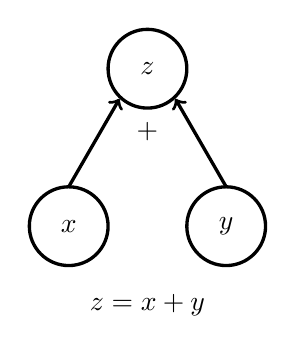
\begin{tikzpicture}
    % Result
    \draw [very thick] (1, 2) circle [radius=0.5cm] node {$z$};

    % Input Nodes
    \draw [very thick] (0, 0) circle [radius=0.5cm] node {$x$};
    \draw [very thick] (2, 0) circle [radius=0.5cm] node {$y$};

    % Edges
    \draw [very thick, ->] (0, 0.5) -- ++(60:1.29);
    \draw [very thick, ->] (2, 0.5) -- ++(120:1.29);

    % Operation Label
    \draw (1, 1.2) node {$+$};

    % Figure Label
    \draw (1, -1) node {$z = x + y$};
  \end{tikzpicture}
  %
  \hspace{0.2cm}
  %
  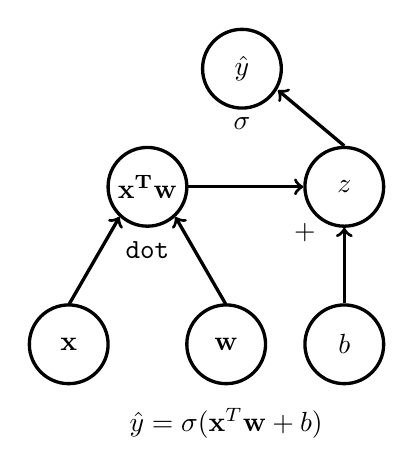
\begin{tikzpicture}
    % x^T w
    \draw [very thick] (1, 2) circle [radius=0.5cm] node {$\mathbf{x^Tw}$};

    % x and weights
    \draw [very thick] (0, 0) circle [radius=0.5cm] node {$\mathbf{x}$};
    \draw [very thick] (2, 0) circle [radius=0.5cm] node {$\mathbf{w}$};

    % Edges
    \draw [very thick, ->] (0, 0.5) -- ++(60:1.29);
    \draw [very thick, ->] (2, 0.5) -- ++(120:1.29);

    % Operation Label
    \draw (1, 1.2) node {\texttt{dot}};

    % Bias
    \draw [very thick] (3.5, 0) circle [radius=0.5cm] node {$b$};

    % z = (x^T w) + b
    \draw [very thick] (3.5, 2) circle [radius=0.5cm] node {$z$};

    % Operation label
    \draw (3, 1.42) node {$+$};

    % Edges
    \draw [very thick, ->] (3.5, 0.52) -- (3.5, 1.48);
    \draw [very thick, ->] (1.52, 2) -- (2.98, 2);

    % Sigmoid
    \draw [very thick] (2.2, 3.5) circle [radius=0.5] node {$\hat{y}$};

    % Operation label
    \draw (2.2, 2.8) node {$\sigma$};

    % Edge
    \draw [very thick, ->] (3.5, 2.52) -- ++(140:1.1cm);


    % Figure Label
    \draw (2, -1) node {$\hat{y} = \sigma(\mathbf{x}^T \mathbf{w} + b)$};
  \end{tikzpicture}
  \label{fig:graphs}
  \caption{Examples of computational graphs. The left graph displays a very
    simple computation, consisting of just an addition of the two input
    variables $x$ and $y$. In this case, $z$ is the result of the operation $+$,
    as the annotation suggests. The right graph shows a more complex example of
    computing a logistic regression variable $\hat{y}$ in dependence of some
    example vector $\mathbf{x}$, weight vector $\mathbf{w}$ as well as a scalar
    bias $b$. As can be seen in the graph, $\hat{y}$ is the result of the
    \emph{sigmoid} function $\sigma$, also known as the \emph{logistic}
    function.}
\end{figure}

\subsubsection{Operations}\label{sec:model-graphs-ops}

The major benefit of representing an algorithm in form of a graph is not only
the intuitive (visual) expression of dependencies between units of a
computational model, but also the fact that the definition of a \emph{node}
within the graph can be kept very general. In TensorFlow, nodes represent
\emph{operations}, which in turn express the combination or transformation of
data flowing through the graph \cite{tensorflow}. An operation can have
\emph{zero or more} inputs and produce \emph{zero or more} outputs. As such, an
operation may represent a mathematical equation, a variable or constant, a
control-flow directive, a file I/O operation or even a network communication
port. It may seem unintuitive that an operation, which the reader may associate
with a \emph{function} in the mathematical sense, can represent a constant or
variable. However, a constant may be thought of as an operation that takes no
inputs and always produces the same output corresponding to the constant it
represents. Analogously, a variable is really just an operation taking no input
and producing the current state or value of that variable. Table \ref{tab:ops}
gives an overview of different kinds of operations that may be declared in a
TensorFlow graph.

\begin{table}[h!]
  \begin{tabular}{ll}
    \textbf{Category} & \textbf{Examples}
    \\ \toprule
    Elementwise operations & \texttt{Add}, \texttt{Mul}, \texttt{Exp}
    \\
    Matrix operations & \texttt{MatMul}, \texttt{MatrixInverse}
    \\
    Value-producing operations & \texttt{Constant}, \texttt{Variable}
    \\
    Neural-network units & \texttt{SoftMax}, \texttt{ReLU}, \texttt{Conv2D}
    \\
    Checkpoint operations & \texttt{Save}, \texttt{Restore}
    \end{tabular}
    \label{tab:ops}
    \caption{Examples for TensorFlow operations \cite{tensorflow}.}
\end{table}

Any operation must be backed by an associated implementation. In
\cite{tensorflow} such an implementation is referred to as the operation's
\emph{kernel}. A particular kernel is always specifically built for execution on
a certain kind of device, such as a CPU, GPU or other hardware unit.

\subsubsection{Tensors}\label{sec:model-graphs-tensors}

In Tensorflow, edges represent data flowing from one operation to another and
are referred to as \emph{tensors}. A tensor is a multi-dimensional collection of
homogenous values with a fixed, static type. The number of dimensions of a
tensor is termed its \emph{rank}. A tensor's \emph{shape} is the tuple
describing the size, i.e. the number of components, of the tensor in each
dimension. In the mathematical sense, a tensor is the generalization of
two-dimensional matrices, one-dimensional vectors and also scalars, which are
simply tensors of rank zero.

In terms of the computational graph, a tensor can be seen as a \emph{symbolic
  handle} to one of the outputs of an operation. A tensor itself does not hold
or store values in memory, but provides only an interface for retrieving the
value referenced by the tensor. When creating an operation in the TensorFlow
programming environment, such as for the expression $x + y$, a tensor object is
returned. This tensor may then be supplied as input to other computations,
thereby connecting the source and destination operations with an edge. By these
means, data flows through a TensorFlow graph.

\subsubsection{Variables}\label{sec:model-graphs-vars}

In a typical situation, such as when performing stochastic gradient descent
(SGD), the graph of a machine-learning model is executed from start to end
multiple times for a single experiment. Between two such invocations, the
majority of tensors in the graph are destroyed and do not persist. However, it
is often necessary to maintain state across evaluations of the graph, such as
for the weights and parameters of a neural-network. Most often, one wishes to
update or \emph{train} this shared state either manually or as part of the
execution of the graph. For this purpose, there exist \emph{variables} in
TensorFlow, which are simply special operations that can be added to the
computational graph.

In detail, variables can be described as persistent, mutable handles to
in-memory buffers storing tensors. As such, variables are characterized by a
certain shape and a fixed type. To manipulate and update variables manually (as
opposed to implicitly by certain library routines), TensorFlow provides the
\texttt{assign} family of graph operations.

When creating a variable node for a TensorFlow graph, one must always supply a
tensor with which the variable is initialized upon graph execution. The shape
and data-type of the variable is then deduced from this
initializer. Interestingly, the variable iself does not store this initial
tensor. Rather, constructing a variable results in the addition of \emph{three}
distinct nodes to the graph:

\begin{enumerate}
  \item The actual variable node, holding the mutable state.
  \item An operation producing the initial value, often a constant.
  \item An \emph{initializer} operation, that \texttt{assign}s the initial value
    to the variable tensor upon evaluation of the graph.
\end{enumerate}

An example for this is given in Figure \ref{fig:variable}.

\begin{figure}[h!]
  \centering
    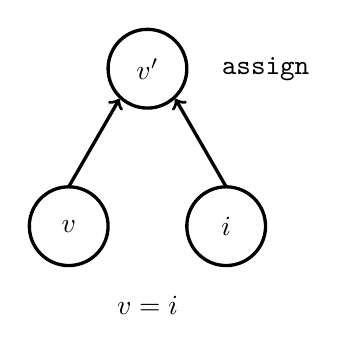
\begin{tikzpicture}
    % Result
    \draw [very thick] (1, 2) circle [radius=0.5cm] node {$v'$};

    % Input Nodes
    \draw [very thick] (0, 0) circle [radius=0.5cm] node {$v$};
    \draw [very thick] (2, 0) circle [radius=0.5cm] node {$i$};

    % Edges
    \draw [very thick, ->] (0, 0.5) -- ++(60:1.29);
    \draw [very thick, ->] (2, 0.5) -- ++(120:1.29);

    % Operation Label
    \draw (2.5, 2) node {\texttt{assign}};

    % Figure Label
    \draw (1, -1) node {$v = i$};
  \end{tikzpicture}
  \label{fig:variable}
  \caption{The three nodes that are added to the computational graph for every
    variable definition. The first, $v$, is the variable operation that holds a
    mutable in-memory buffer containing the value-tensor of the variable. The
    second, $i$, is the node producing the initial value for the variable, which
    can be any tensor (that is, the result of any operation). Lastly, the
    \texttt{assign} node will set the variable to the initializer's value when
    executed. The \texttt{assign} node also produces a tensor referencing the
    initialized value $v'$ of the variable, such that it may be connected to
    other nodes as necessary (e.g. when using a variable as the initializer for
    another variable). }
\end{figure}

\subsubsection{Sessions}\label{sec:model-graphs-sessions}

In TensorFlow, the execution of operations and the evalution of tensors may only
be performed in a special environment referred to as \emph{session}. One of the
responsibilities of a session is to encapsulate the allocation and management of
resources such as variable buffers. Moreover, the \texttt{Session} interface of
the TensorFlow library provides a \texttt{run} routine, which is the primary
entry-point for executing parts or the entirety of a computational graph. This
method takes as input the nodes in the graph whose tensors should be computed
and returned. Moreover, an optional mapping from arbitrary nodes in the graph to
respective replacement values --- referred to as \emph{feed nodes} --- may be
supplied to \texttt{run} as well \cite{tensorflow}.

Upon invocation of \texttt{run}, TensorFlow will start at the requested output
nodes and work backwards, examining the graph dependencies and computing the
full transitive closure of all nodes that must be executed. These nodes may then
be assigned to one or many physical execution units (CPUs, GPUs etc.) on one or
many machines. The rules by which this assignment takes place are determined by
TensorFlow's \emph{placement algorithm}, discussed in detail in Subsection
\ref{subsec:execmodel}, Moreover, as there exists the possibility to specify
explicit orderings of node evaluations, called \emph{control dependencies}, the
execution algorithm will ensure that these dependencies are maintained.

\subsection{Execution Model}\label{sec:model-exec}

\subsubsection{Devices}\label{sec:model-exec-devices}

What are devices? GPUs, cpus, tpus(!)

\subsubsection{Placement Algorithm}\label{sec:model-exec-placement}

\subsubsection{Single-Device Execution}\label{sec:model-exec-single}

\subsubsection{Multi-Device Execution}\label{sec:model-exec-many}

\subsection{Optimizations}\label{sec:model-optim}

\subsubsection{Common-Subexpression Elemination}\label{sec:model-optim-common}

\subsubsection{Scheduling}\label{sec:model-optim-schedule}

\subsubsection{Lossy Compression}\label{sec:model-optim-lossy}

\subsubsection{Asynchronous Kernels}\label{sec:model-optim-async}

\subsection{Extensions}\label{sec:model-ext}

\subsubsection{Backpropagation Nodes}\label{sec:model-ext-backprop}

\subsubsection{Checkpoints}\label{sec:model-ext-check}

\subsubsection{Control-Flow}\label{sec:model-ext-flow}

\subsubsection{Queues}\label{sec:model-ext-queues}

%%% Local Variables:
%%% mode: latex
%%% TeX-master: "../paper"
%%% End: